\chapter{Diagnostic et Pronostic des Roulements avec les Réseaux de Neurones}
\label{chapter:diagnostic-and-prognostic-of-bearings-using-neural-networks}
\chapterintrobox{La surveillance des vibrations est vitale pour de nombreux systèmes industriels. Les mesures des vibrations contiennent des informations très utiles sur l'état de santé des équipements et les types de défauts. Néanmoins, obtenir des informations à partir de ces signaux dans des applications réelles se révèle être un processus complexe. Cela est principalement dû à la complexité du problème. Ce chapitre présente plusieurs approches pour le diagnostic et le pronostic des défauts de roulements à l'aide de réseaux de neurones convolutifs.}

\section{Etude de cas: Diagnostique des roulements}%
\label{sec:etude_de_cas_diagnostique_des_roulements}

\begin{wrapfigure}[14]{r}{0.5\textwidth}
    \centering
	\begin{tikzpicture}
	\node (outer) at (3.5,1.2) {\makecell{\small Outer\\Race}};
	\node (inner) at (3.5,0) {\makecell{\small Inner\\Race}};
	\node (ball) at (3.5,-1.2) {\makecell{\small Ball\\(in cage)}};
	
	\node (outer2) at (1.3,1.2) {};
	\node (inner2) at (.3,0) {};
	\node (ball2) at (-.5,-1.2) {};

	\node[inner sep=0] (image) at (0,0) {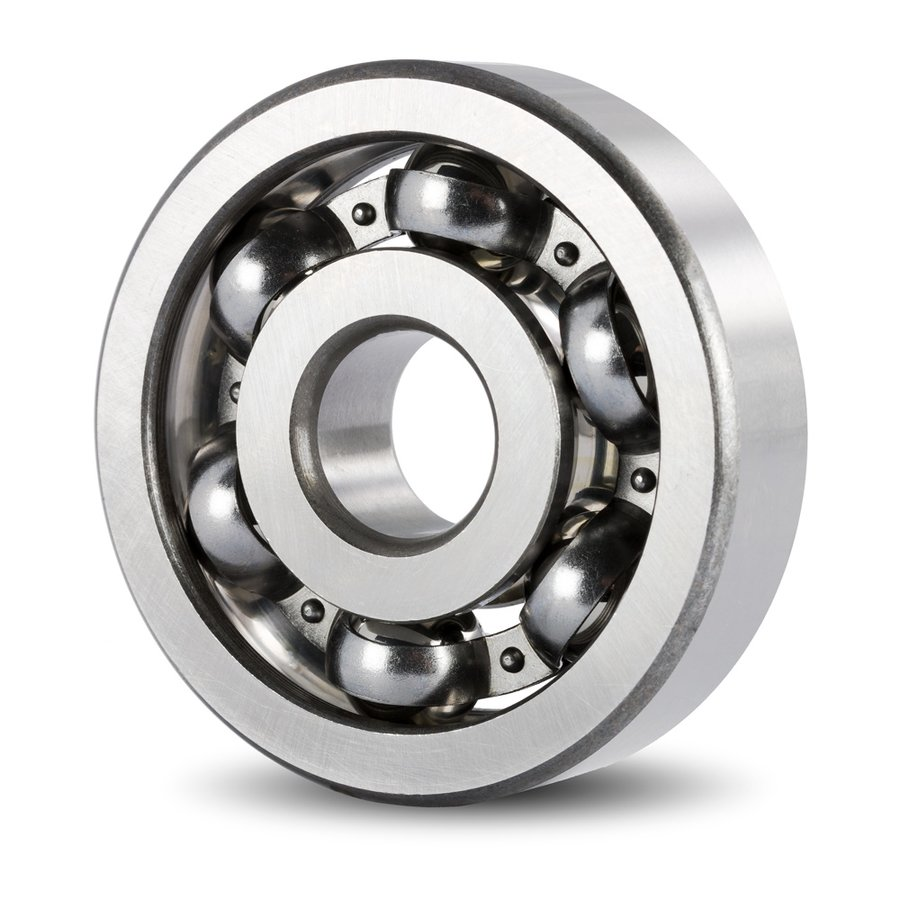
\includegraphics[width=0.35\textwidth]{figures/skf.jpg}};

	\draw [|->,  thick, red] (outer.west) -- (outer2);
	\draw [|->,  thick, red] (ball) -- (ball2);
	\draw [|->,  thick, red] (inner) -- (inner2);
\end{tikzpicture}
	\caption{Composants d'un roulement}
    \label{figure:skf-bearing-components}    
\end{wrapfigure}

Les données utilisées dans cette section sont des données de vibrations des roulements fournies par Case Western Reserve University (CWRU). Les roulements utilisés dans le test sont des roulements à billes SKF. La figure \ref{figure:skf-bearing-components} montre les différents composants d'un roulement à billes standard. L'essai a été réalisé là où les roulements supportent l'arbre d'un moteur de 2 chevaux dans différentes conditions de charge. 

Les roulements d'essai possèdent des défauts ponctuels qui ont été introduits par électroérosion avec des diamètres de défaut de 0,18 mm, 0,36 mm, 0,53 mm, 0,71 mm et 1,02 mm. Ces défauts ont été introduits dans la bille et les chemins de roulement intérieurs et extérieurs du roulement. Des roulements SKF ont été utilisés pour les défauts de 0,18 mm, 0,36 mm et 0,53 mm, et des roulements équivalents NTN ont été utilisés pour les défauts de 0,71 mm et 1,02 mm. Le tableau \ref{table:cwru-bearings-specification} contient les dimensions des modèles de roulements SKF utilisés et les fréquences correspondantes (en multiples de RPM) associées aux différents types de défauts.

\begin{table}[H]
	\centering
	\begin{tabu}{cc|[1.5pt]cc}
		\tabucline[1.5pt]{-} 
		Dimension		&	Valeur (mm)	&	Défaut 			& Fréquence ($\times$RPM Hz)	\\
		\hline
		Diamètre intérieur	&	25.00		& Chemin intérieur 		& 5.4152\\
		Diamètre extérieur&	52.00		& Chemin extérieur 		& 3.5848 \\
		Epaisseur 		&	15.00		& Cage		& 0.3983 \\
		Diamètre du pas	&	08.03		& Bille	& 4.7135\\
		\tabucline[1.5pt]{-} 
	\end{tabu}
	\caption{Dimensions des roulements CWRU et les fréquences de défaults}
	\label{table:cwru-bearings-specification}
\end{table}

\subsection{Génération de données à partir de vibration}
Les données de vibration non traitées ne peuvent pas être utilisées directement pour entraîner un réseau de neurones. Ce chapitre utilise l'approche proposée dans \cite{Wen2018} pour convertir les données de vibration non traitées en images. La figure \ref{fig:cw_bearings_data_generation} montre le principe de génération de données où les signaux de vibration à une dimension sont convertis en matrices à deux dimensions (images) en transformant des morceaux de longueur 4096 en matrices de 64$\times$64.

\begin{figure}[h]
	\centering
	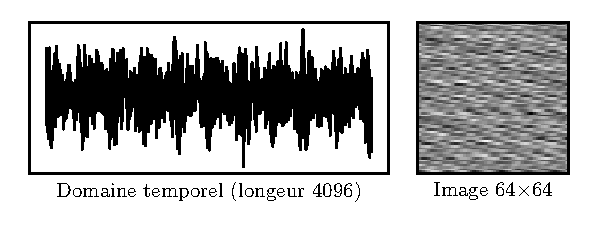
\includegraphics{figures/cw_bearings_data_generation_fr.pdf}
	\caption{Génération de données par conversion du signal en images 64$\times$64}
	\label{fig:cw_bearings_data_generation}
\end{figure}

Comme mentionné précédemment, plusieurs essais ont été réalisés avec différents types de défauts de roulements (c'est-à-dire des défauts de billes, de chemins de roulement intérieurs et extérieurs) avec différents diamètres de défaut. Les signaux des différents tests sont transformés en images pour servir d'entrée à un réseau de neurones convolutif qui sera entraîné à classer les différents signaux dans les types de défauts correspondants et leurs diamètres. Les signaux sont répartis en 10 classes : trois types de défauts différents et pour chaque type de défaut, il y a trois diamètres de défaut différents, plus un signal de base normal qui appartient au roulement sain. La figure \ref{fig:bearings_faults_samples} montre quelques échantillons des signaux transformés des neuf différents types de défaut/diamètres : 

\begin{figure}[h]
    \centering
	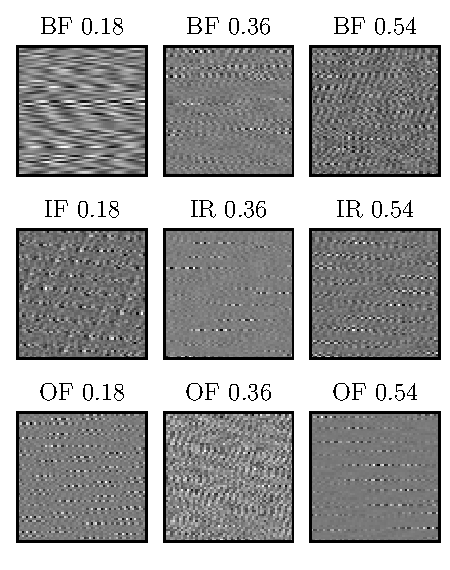
\includegraphics{figures/cw_bearings_faults_samples.pdf}
    \caption{Signaux convertis de différents types de défauts}
    \label{fig:bearings_faults_samples}
\end{figure}

Les signaux des différents types de défauts ont des longueurs variables, ce qui se traduit par un nombre différent d'images synthétisées par type de défaut. Le nombre d'images par type de défaut (classe) est donné par l'équation \ref{equation:labels-per-class} :

\begin{equation}
	N=floor \left(\frac{\text{signal length}}{64\times64}\right)
	\label{equation:labels-per-class}
\end{equation}

Le nombre d'images correspondant à chaque classe est indiqué dans le tableau \ref{table:cw-classes-count}:
